% !TEX encoding = UTF-8 Unicode
% ÄÖÜ ß äöü

The aim of this project was to design an interactive environment on a tablet computer 
that allows the user to learn simple facts about the formalism of propositional logic 
and standard transformations of Boolean functions. 
The environment was meant to be self-explanatory. 

The core of this concept builds on tutorials with exercises 
and a playground where the learned knowledge can be used in different modes. 
A glossary of terms and a formula calculator (BoolTool) to check formulas will support the user in their learning.

\section{Tutorials}

Ny$\bar{a}$ya for iPad covers syntax and semantics of propositional logic, 
but only some basic rules of natural deduction. 
It introduces normal forms, truth tables and binary decision diagrams 
as different but equivalent representations of Boolean functions.

The structure of the tutorials and the content of the exercises are heavily based on the according sections of the book  
{\em Logic in Computer Science} \cite{Huth:2004:LCS:975331} by M.~Huth and M.~Ryan.
Additional content was taken from the lecture {\em Logic} \cite{Middeldorp:2012:LICS} by {A. Middeldorp}.


\begin{table}[htdp]
\begin{center}
\begin{lstlisting}[mathescape,firstnumber=5]
  <array> 		<!-- root with title and sections -->
    <string>Tutorials</string> 					<!-- title -->
    <array>			<!-- section with section title and tutorials-->
      <string>Introduction</string> 				<!-- section title -->
      <array>		<!-- tutorial with title and id -->
        <string>Motivation</string> 	<!-- tutorial title -->
        <string>11</string> 						<!-- tutorial id -->
      </array>
		$\square$
\end{lstlisting}
\caption{Tutorials.plist – the configuration file for all tutorials}
\label{tab:TUTORIALPLIST}
\end{center}
\end{table}%

General and specific configurations for the tutorials and additional content for the exercises 
are stored in simple property lists\footnote{
\href{http://www.apple.com/DTDs/PropertyList-1.0.dtd}{http://www.apple.com/DTDs/PropertyList-1.0.dtd}
(see \tabref{tab:PLISTDTD}). }, 
which are xml-files with some basic data types for data and collections, 
that can be easily read and interpreted by different programs.
The file “Tutorials.plist” (see \tabref{tab:TUTORIALPLIST}) 
provides the basic data about available tutorial sections and tutorial titles 
to build a navigation menu programmatically.

Every tutorial includes a teaching part with examples (html-files in utf-8 encoding) 
and an interactive knowledge checker with exercises, 
where the user gets immediate feedback. 
Every interactive part will present some instructions to master the task.

\subsection{Introduction}

The first tutorial section with four tutorials 
(\hyperref[tut:11]{11}, 
\hyperref[tut:12]{12}, 
\hyperref[tut:13]{13},
\hyperref[tut:14]{14}) 
gives an informal introduction to modeling, 
i.e. the translation from sentences in natural language to sentences in the formal language of propositional logic.

The content file “QA1.plist” (see \tabref{tab:QA1PLIST}) contains
an array (starts at line 5) 
of arrays that include sentences and sample solutions 
(the first exercise starts at line 6). 
The first string is the sample sentence (at line 7), 
which must be analyzed by the user
and the following strings are sample solutions for different exercises. 

\begin{table}[htdp]
\begin{center}
\begin{lstlisting}[firstnumber=5]
<array>
  <array> 
    <string>If the barometer falls, then it will rain.</string>
    <string>if p then q</string>
    <string>the barometer falls; it will rain</string>
    <string>p $\rightarrow$ q</string>
  </array>
$\square$
\end{lstlisting}
\caption{QA1.plist – content file for the first three tutorials}
\label{tab:QA1PLIST}
\end{center}
\end{table}%

Each tutorial has its own configuration file 
(see \tabref{tab:11PLIST})
with a dictionary that
describes the task and defines the index of the sample solution,
with which the user's answer will be checked with some tolerance.

\begin{table}[htdp]
\begin{center}
\begin{lstlisting}[firstnumber=5]
<dict>
  <key>questionLabelText</key>
  <string>Guess the structure …</string>
  <key>answerLabelText</key>
  <string>Use … </string>
   <key>solutionLabelText</key>
   <string>Sample solution</string>
   <key>questionsFile</key>
   <string>QA1</string>
   <key>solutionIndex</key>
   <integer>1</integer>
</dict>
\end{lstlisting}
\caption{11.plist – configuration file for the first exercise}
\label{tab:11PLIST}
\end{center}
\end{table}%

\subsubsection{Applications}
\label{tut:11}

(11) The aim of logic in general is to reason about situations \cite{Huth:2004:LCS:975331}. 
In this tutorial it is shown, how two different paragraphs in natural language 
can be reduced to the same formal sentence “If p and not q, then r. Not r. p. Therefore, q“. 
If the reasoning is correct, the user can use it in both situations. 

In the interactive part the user has to ‘guess’ the formal structure of composite sentences in natural language. 
The sentence 
\verb+‘If the barometer falls,+ \verb+then it will rain’+ 
from line 7 of \verb+QA1.plist+ (\tabref{tab:QA1PLIST})
has to be translated into
\verb+‘if p then q’+ from line 8 (the solution index is defined as 1 in \verb+11.plist+, see \tabref{tab:11PLIST}).

\subsubsection{Propositions}
\label{tut:12}

(12) The concept of propositions – simple declarative sentences – 
as indivisible building blocks of propositional logic 
is explained in more detail. Some counter-examples are presented 
and the ambiguity of natural language is demonstrated.

The user has to find the propositions in composite sentences. 
The correct answer for 
\verb+‘If the barometer falls,+ \verb+then it will rain’+ 
would be  
\verb+‘the barometer falls; it will rain’+ 
from line 9 
(the solution index is defined as 2 in \verb+12.plist+).


\subsubsection{Connectives}
\label{tut:13}

(13) The basic symbols of propositional logic to connect propositions are introduced. 
“$\rightarrow$”, “$\neg$”, “$\wedge$”, and “$\vee$”
 will replace “if then”, “not”, “and” and “or”. 

For the sentence
\verb+‘If the barometer falls,+ \verb+then it will rain’+ 
a correct answer is
\verb+‘p+ $\rightarrow$ \verb+q’+ 
from line 10 
(the solution index is defined as 3 in \verb+13.plist+),
but 
‘$\neg p \vee q$’ would be accepted too.

\subsubsection{Limits}
\label{tut:14}

(14) Some examples are given to demonstrate that not every situation can modeled in propositional logic.

The user has to ‘guess’ whether sentences in natural language are suitable for propositional logic.

\subsection{Syntax}

After the informal introduction into the atoms and connectives of propositional logic, 
the formal aspects of propositional logic will be introduced to the user.

The content of these exercises will be generated by the app and the user's solution will be checked without tolerance.

\subsubsection{Definition}
\label{tut:21}

(21) The definition of well formed formulas is explained. 

\begin{table}[htdp]
\begin{center}
\begin{tabular}{rcccccccccc}
$P$	&$::=$	&$p$ 	
	&|		& $(\neg P)$ 
	&|		&  $(P \wedge P)$ 
	&|		&  $(P \vee P)$ 
	&|		&  $(P \rightarrow P)$ \\
\end{tabular}
\caption{Grammar with mandatory parentheses}
\label{tab:BNFGRPA}
\end{center}
\end{table}

The user has to check whether a formula matches the strict definition of 
a propositional formula (see \tabref{tab:BNFGRPA}).
If the formula is well formed, the user has to write down the name of the root connective, i.e
negation, conjunction, disjunction or implication. 
If the formula is not well formed, the user has to leave the answer field empty.

\subsubsection{Conventions}
\label{tut:22}

(22) The conventions of precedences and associativity  of connectives to save parentheses are introduced. 

The user has to rewrite formulas from strict syntax to formulas using conventions and vice versa.

\begin{table}[htdp]
\begin{center}
\begin{tabular}{rcccl}
$P$		&$::=$ & $D$ &|& $D \rightarrow P$\\
$D$		&$::=$ & $C$ &|& $D \vee C$			\\
$C$		&$::=$ & $N$ &|& $C \wedge N$ 		\\
$N$		&$::=$ & $T$ &|& $\neg N$ 			\\
$T$		&$::=$ & $p$ &|& $(P)$
\end{tabular}
\caption{Grammar with precedence and associativity}
\label{tab:BNFGRPR}
\end{center}
\end{table}

%\begin{table}[htdp]
%\begin{center}
%\begin{tabular}{rcl}
%P		&$::=$ & D [ $\rightarrow$ P ]\\
%D		&$::=$ & C \{ $\vee$ C \}\\
%C		&$::=$ & N  \{ $\wedge$ N \} \\
%N		&$::=$ & $\neg$N | p | (P) \\
%\end{tabular}
%\caption{EBNF Grammar (with precedences)}
%\label{tab:BNF}
%\end{center}
%\end{table}

\subsubsection{Sub-formulas}
\label{tut:23}

(23) Sub-formulas (starting from atoms) are used to build bigger formulas. Big formulas are build from many sub-formulas.

The user have to extract the set of sub-formulas from composite formulas. 
A correct answer for 
‘$a \vee b \wedge c$’ would be
‘$a,b,c,b\wedge c, a \vee b \wedge c$‘. 
The order of the sub-formulas does not matter and the user can use parentheses as they like it.
But no sub-formula may occur more than once.

\subsubsection{Syntax Trees}
\label{tut:24}

(24) Syntax trees as graphical representation of well formed formulas are introduced. 

The user has to write formulas for presented syntax trees. They can use parentheses as they like – still the formulas has to match the syntax trees exactly. ‘$a \vee b$’ does not match the syntax tree representing ‘$b \vee a$’, where the node ‘$a$’ is on the right branch of the node ‘$\vee$’.

\subsubsection{Top and Bottom}
\label{tut:25}

(25) Some natural deduction rules are introduced. 
“$\top$” (top) and “$ \bot$” (bottom) are defined
as abbreviations of conjunctions and disjunctions 
of formulas with their negation (tautologies and contradictions, \tabref{tab:TopBottom}).

CIM

\begin{table}[htdp]
\begin{center}
\begin{tabular}{c|c|c|c}
$\neg P \vee P$&$P \vee \neg P$  & $\neg P \wedge P$ & $P \wedge \neg P$ \\
\hline
$\top$ & $\top$ & $ \bot$&$ \bot$\\
\end{tabular}
\caption{tautologies and contradictions}
\label{tab:TopBottom}
\end{center}
\end{table}%

%\subsubsection{Simplifying formulas – basic natural deduction rules}
%\label{tut:206}

%(206) The tutorial teaches the simplifying of conjunctions and disjunctions with top, bottom and/or the same sub formulas.
%
%
%
\begin{table}[htdp]
\begin{center}
\begin{tabular}{c|c|c|c|c}
$\neg \neg P$ & $P \vee P$ & $P \wedge P$ & $P \vee Q$ & $P \wedge Q$\\
\hline
$P$ & $P$ & $P$ & $Q \vee P$ & $Q \wedge P$\\
\end{tabular}
\caption{basic rules}
\label{tab:BasicRules}
\end{center}
\end{table}
%
%The user has to rewrite some formulas eleminating 
%top, bottom, double negations, conjunctions and disjunctions 
%by using rules from 
%\tabref{tab:TopBottom} and \tabref{tab:BasicRules}.

%\subsubsection{Conjunctive Normal Form} 
%\label{tut:207}
%(207) The syntax of formulas in conjunctive normal form is introduced (\tabref{tab:CNF}) and explained.
%It is shown that some formulas in cnf can be simplified to top.

%
%The user has to guess if a presented formula is in conjunctive normal form
%and if it can be simplified to top ($\top$).


%\subsubsection{Disjunctive Normal Form} 
%\label{tut:208}
%(208) The syntax of formulas in disjunctive normal form is introduced (\tabref{tab:DNF}) and explained.
%It is shown that some formulas in dnf can be simplified to bottom.

%
%The user has to guess if a presented formula is in disjunctive normal form
%and if it can be simplified to bottom ($\bot$).


\subsection{Semantics}

After the introduction of well formed formulas the meaning of logical connectives is defined.

\subsubsection{Valuation}
\label{tut:31}
(31)
The truth assignment for atoms $(p,q,r,…)$ is introduced. 
The extended valuation for negation, conjunction, disjunction and implication is defined.
The valuation of arbitrary formulas by evaluating all sub-formulas is described.

The user has to guess or calculate the evaluation of a given formula with a given truth assignment of the atoms of the formula.

\subsubsection{Truth Tables}
\label{tut:32}
(32)
The concept of truth tables is explained and demonstrated with the basic connectives. 
The valuation of arbitrary formulas by evaluating all sub-formulas is demonstrated again.

The user has to fill in truth tables for formulas with a maximum of three atoms.

\subsubsection{Entailment and Equivalence}
\label{tut:33}
(33) Semantic entailment and equivalence is defined and explained with various examples.

The user has to guess or calculate whether a given semantic entailment or equivalence holds. 

\subsubsection{Satisfiability and Validity}
\label{tut:34}
(34) The properties satisfiability and validity of propositional formulas are defined and demonstrated. 
The relationship of these properties with top and bottom is mentioned. 

The user has to guess or calculate whether a given formula is satisfiable or valid.

\subsection{Normal Forms}

The advantages of propositional formulas in special shapes will be emphasized.
%\hyperref[tut:207]{CNFs} and \hyperref[tut:208]{DNFs} are already defined
%in \tabref{tab:CNF} and \tabref{tab:DNF}.
The definitions of implication free forms, negation normal form, 
conjunctive normal forms and disjunctive normal forms will be provided. 
An receipt to transform arbitrary propositional formulas into specific normal forms will be delivered.
Rules to detect satisfiability or validity from normal forms will be mentioned.

\subsubsection{Implication Free Form}
\label{tut:41}
(41)
By removing the rule for $P$ from the grammar in \tabref{tab:BNFGRPR} 
the grammar for implication free forms is defined  
(see \tabref{tab:BNFGRIFF}). 

\begin{table}[htdp]
\begin{center}
\begin{tabular}{rcccl}
$D$		&$::=$ & $C$ &|& $C \vee D$			\\
$C$		&$::=$ & $N$ &|& $N \wedge C$ 		\\
$N$		&$::=$ & $T$ &|& $\neg N$ 			\\
$T$		&$::=$ & $p$ &|& $(D)$
\end{tabular}
\caption{Grammar without implications}
\label{tab:BNFGRIFF}
\end{center}
\end{table}

The equivalence transformation (see \tabref{tab:ET_IFF}) 
for removing implications is presented
and proved with a truth table. 

\begin{table}[htdp]
\begin{center}
\begin{tabular}{r}
$P \rightarrow Q$ \\ 
————\\
$\neg P \;\vee\; Q$
\end{tabular}
\caption{Equivalence transformation towards implication free form}
\label{tab:ET_IFF}
\end{center}
\end{table}

The user has to check whether a given formula is implication free.
If the formula is not implication free the user has to transform it into an implication free form
using the equivalence transformation.

\subsubsection{Negation Normal Form}
\label{tut:42}

(42)
By removing all  rules for arbitrary negations, the negation normal form is defined
 (\tabref{tab:BNFGRNNF}). 

\begin{table}[htdp]
\begin{center}
\begin{tabular}{rcccl}
$D$		&$::=$ & $C$ 		&|& 	$C \vee D$\\
$C$		&$::=$ & $N$ 		&|& 	$N \wedge C$ \\
$N$		&$::=$ & $(D)$ 	&|& 	$L$\\
$L$		&$::=$ & $p $ 		&|& 	$\neg p$
\end{tabular}
\caption{Grammar for negation normal form}
\label{tab:BNFGRNNF}
\end{center}
\end{table}

The equivalence transformations to transform negations of conjunctions,
negations of disjunctions, 
and double negations (see \tabref{tab:ET_NNF})
into negation normal forms are presented 
and proved with truth tables.

\begin{table}[htdp]
\begin{center}
\begin{tabular}{ccr}
$\neg (P \wedge Q) $&$ \neg (P \vee Q)$&$ \neg \neg P$\\
————— & —————& ———\\
$\neg P \vee \neg Q$&$\neg P \wedge \neg Q$&$P$
\end{tabular}
\caption{Equivalence transformations towards negation normal form}
\label{tab:ET_NNF}
\end{center}
\end{table}

The user has to check whether a given formula is in negation normal form.
If the formula is not in negation normal form
the user has to transform it into negation normal form.

\subsubsection{Conjunctive Normal Form}
\label{tut:43}

(43) A formula in conjunctive normal form is a conjunctive concatenation of disjunctive clauses.
A disjunctive clause is a disjunctive concatenation of literals. 
A literal is an atom or the negation of an atom. 

\begin{table}[htdp]
\begin{center}
\begin{tabular}{rcccl}
$C$	&$::=$ & $(D)$ 	&$|$ & $(D) \wedge C$\\
$D$	&$::=$ & $L$ 	&$|$ & $L \vee D$\\
$L$	&$::=$ & $p$ 	&$|$ & $\neg p$ 
\end{tabular}
\caption{Grammar for conjunctive normal form}
\label{tab:CNF}
\end{center}
\end{table}

The user learns the distribution of disjunctions over conjunctions (\tabref{tab:ET_CNF}).

\begin{table}[htdp]
\begin{center}
\begin{tabular}{cc}
$P \vee (Q \wedge R)$ & $(P \wedge Q) \vee R$\\
———————— & ————————\\
$(P\vee Q) \wedge (P\vee R)$ & $(P\vee R) \wedge (Q\vee R)$
\end{tabular}
\caption{Equivalence transformations towards conjunctive normal form}
\label{tab:ET_CNF}
\end{center}
\end{table}

The user has to rewrite formulas to a conjunctive normal form.  
The presented formula is in negation normal form 
but may already be in conjunctive normal form.


\subsubsection{Disjunctive Normal Form}
\label{tut:44}

(44) A formula in disjunctive normal form is a disjunctive concatenation of conjunctive clauses.
A conjunctive clause is a conjunctive concatenation of literals. 
A literal is an atom or the negation of an atom. 

\begin{table}[htdp]
\begin{center}
\begin{tabular}{rcccl}
$D$	&$::=$ & $C$ 	&$|$ & $C \;\vee D$\\
$C$	&$::=$ & $L$ 	&$|$ & $L \wedge D$\\
$L$	&$::=$ & $p$ 	&$|$ & $\neg p$
\end{tabular}
\caption{Grammar for disjunctive normal form}
\label{tab:DNF}
\end{center}
\end{table}

The user learns the distribution of conjunctions over disjunctions (\tabref{tab:ET_DNF}).

\begin{table}[htdp]
\begin{center}
\begin{tabular}{cc}
$P \wedge (Q \vee R)$ 			& $(P \wedge Q) \wedge R$\\
———————— & ————————\\
$(P\wedge Q) \vee (P\wedge Q)$ 	& $(P\wedge R) \vee (Q\wedge R)$
\end{tabular}
\caption{Equivalence transformations towards disjunctive normal form}
\label{tab:ET_DNF}
\end{center}
\end{table}

The user has to rewrite formulas to a disjunctive normal form. 
The presented formula is in negation normal form 
but may already be in disjunctive normal form.

%\subsubsection{From general formula to CNF or DNF}
%\label{tut:406}
%(406)
%To combination of the previous techniques to reach a equivalent representation in conjunctive or disjunctive normal form is provided.
%The potential exponential growing of the length of these transformations is demonstrated.
%
%The user has to rewrite formulas to a conjunctive or disjunctive normal form.
%The presented formula is in general form
%but may already be in the demanded normal form.
%
%\subsubsection{Validity of CNF}
%\label{tut:407} 
%(407) 
%If every disjunctive clause contains at least two contemplementary literals.
%then a formula in conjunctive normal form  is valid (a tautology).
%
%The user has to guess or calculate satisfiability of formulas in conjunctive normal form.
%
%\subsubsection{Satisfiability of DNF} 
%\label{tut:408}
%(408) 
%If every conjunctive clause contains at least two contemplementary literals,
%then a formula in disjunctive normal form  is not satisfiable (a contradiction).
%
%The user has to to guess or calculate satisfiability of formulas in disjunctive normal form.

\subsection{Binary Decision Diagrams}

\subsubsection{Boolean functions}
\label{tut:51}

(51) N-ary Boolean functions are introduced as mapping from n-tupels of 0s and 1s to the set ${0,1}$.
The symbols $+,.,\oplus$ for building Boolean expressions are introduced as special representation of
specific unitary and binary Boolean functions.


\subsubsection{Boolean expressions}
\label{tut:52}

(52) The grammar for Boolean expressions is provided. 
The equivalence of Boolean expressions is defined.

\begin{table}[htdp]
\begin{center}
\begin{tabular}{rcccccccccc}
$B$	&$::=$	&$p$ 	
	&|		& $(\overline{B})$ 
	&|		&  $(B \cdot B)$ 
	&|		&  $(B + B)$ 
	&|		&  $(B \oplus B)$ \\
\end{tabular}
\caption{Grammar for Boolean expressions}
\label{tab:BNFGRBE}
\end{center}
\end{table}

The user has to rewrite formulas with propositional symbols into Boolean expressions.
The implication may be a challenge for some users, 
but is doable because the implication free form was introduced 
in an earlier tutorial.

\subsubsection{Binary Decisions}
\label{tut:53}

(53) Binary decision nodes are introduced. 
The valuation of binary decision trees is explained.

The user has to fill in the result nodes in a binary decision tree for a given Boolean expression.

\subsubsection{ROBDD}
\label{tut:54}

(54)

The user has to check whether a binary decision diagram is ordered or reduced.

\section{Playground}

In the playground the user can create arbitrary propositional formulas 
by building syntax trees interactively.
Truth assignments can be applied and will be visualized.
The playground supports a least the following use cases.

\begin{itemize}

\item In the {\em free mode} arbitrary formulas can be created by adding, replacing and removing connectives and atoms. The process starts with an atom, which an be expanded or replaced. 
Connectives can be changed any time, sub-formulas can be reordered.
The smallest possible formula consists of one atom with one symbol from the set $\{ \top, \bot, p, q, r, … \}$.

\item In the {\em locked mode} only equivalence transformations can be applied to nodes (see \tabref{tab:ET:ALL})
– depending on the kind of node. 

\item Truth values can be assigned to leaf nodes, 
which represent the atoms of the corresponding propositional formula. 
By default no truth values are assigned to atoms, which is visualized by a blue color of the node.
A green color represents ‘true’, and a red color ‘false’.
The valuation of connective nodes is calculated automatically 
and displayed using the same blue, green and red colors.

\item Connective nodes of obvious tautologies like
$P \vee \neg P$ or
$P \rightarrow P$ are displayed with a green color – 
independent form the valuation status of any sub-node.

\item Connective nodes of obvious contradictions like $P \wedge \neg P$ are displayed with a red color – 
independent form the valuation status of any sub-node.

\item While working with a syntax tree, the corresponding propositional formula is shown on top of the playground.

\item While selecting a sub-node of the syntax tree – the root of a sub-tree – 
for manipulation the corresponding sub-formula will be highlighted in the corresponding propositional formula.

\end{itemize}


\begin{table}[htdp]
\begin{center}
\begin{tabular}{rcl|rcl}

$P$&$ \TAP{\rightarrow}$&$Q$				&$ $&$\TAP{\neg}$&$\neg P$			\\
\hline
$\neg P $&$ \TAP{\vee}$&$Q$					&$ $&$\TAP{P}$&$ $				\\
\\
$ $&$\TAP{\neg}$&$(P \vee Q)$				&$ $&$ \TAP{\neg}$&$(P \wedge Q)$	\\
\hline
$\neg P$&$\TAP{\wedge}$&$\neg Q$			&$\neg P$&$ \TAP{\vee}$&$\neg Q$	\\
\\
$P$&$\TAP{\vee}$&$P$						&$P$&$ \TAP{\wedge}$&$P$			\\
\hline
$$&$\TAP{P}$&$$							&$$&$ \TAP{P}$&$$					\\
\\
$P$&$\TAP{\vee}$&$\neg P$					&P&$\TAP{\wedge}$&$\neg P$		\\
\hline
$ $&$\TAP{\top}$&$ 	$						&	&$\TAP{\bot}$&$ $				\\
\\
$P$&$\TAP{\vee}$&$\top$					&P	&$\TAP{\wedge}$&$\top$			\\
\hline
$ $&$\TAP{\top}$&$ 	$						&	&$\TAP{P}$&$ $				\\
\\
$P$&$\TAP{\vee}$&$\bot$					&$P$&$ \TAP{\wedge}$&$\bot$		\\
\hline
$ $&$\TAP{P}$&$ $							&$ $&$ \TAP{\bot}$&$ $				\\
\\
$P$&$\TAP{\vee}$&$Q$						&$P$&$ \TAP{\wedge}$&$Q$			\\
\hline
$Q$&$\TAP{\vee}$&$P$						&$Q$&$ \TAP{\wedge}$&$P$			\\
\\
$P$&$\TAP{\vee}$&$(Q\wedge R)$				&$P$&$\TAP{\wedge}$&$(Q\vee R)$			\\
\hline
$(P\vee Q)$&$\TAP{\wedge}$&$(P\vee R)$		&$(P\wedge Q)$&$\TAP{\vee}$&$(P\wedge R)$	\\
\\
$(P\wedge Q)$&$\TAP{\vee}$&$R$				&$(P\vee Q)$&$\TAP{\wedge}$&$R$			\\
\hline
$(P\vee R)$&$\TAP{\wedge}$&$(Q\vee R)$		&$(P\wedge R)$&$\TAP{\vee}$&$(Q\wedge R)$	\\
\\
$P$&$\TAP{\vee}$&$(Q\vee R)$				&$P$&$\TAP{\wedge}$&$(Q\wedge R)$			\\
\hline
$(P\vee Q)$&$\TAP{\vee}$&$R$			&$(P\wedge Q)$&$\TAP{\wedge}$&$R$	\\

\end{tabular}
\caption{Transformations which are offered in locked mode}
\label{tab:ET:ALL}
\end{center}
\end{table}%

%\begin{table}[htdp]
%\begin{center}
%\begin{tabular}{rcl|rcl}
%
%$P$&$ \TAP{\leftrightarrow}$&$Q$					&$P$&$ \TAP{\veebar}$&$Q$			\\
%\hline
%$P \rightarrow Q $&$ \TAP{\wedge}$&$Q \rightarrow P$	&$\neg(P \rightarrow Q) $&$ \TAP{\vee}$&$\neg (Q \rightarrow P)$				\\
%
%\end{tabular}
%\caption{Additional transformations in locked mode}
%\label{tab:addnf}
%\end{center}
%\end{table}%


\section{Glossary}

Terms, definitions and truth tables from the tutorials are listed in the glossary in a searchable and hyperlinked form.

\section{BoolTool}

The interactive environment have to contain the functionality of the \href{web fronted} of BoolTool.

\subsection{Input}

As minimum the embedded BoolTool must support Latin letters as identifiers for atoms, 
\verb#T# (top), 
\verb#F# (bottom),
\verb#!# (negation), 
\verb#&# (conjunction),
\verb#+# (disjunction),
\verb#># (implication) and 
\verb#^# (exclusive disjunction), because these ASCII-symbols can be found on almost every keyboard.

Standard symbols “$ \neg \vee \wedge \rightarrow $” 
and additional symbols of propositional logic and Boolean expressions
should be accepted too (see \tabref{tab:BASICSYMBOLS}) 
to make extended or custom keyboards more useful.
A limitation of the Latin characters for identifiers should be avoided (\figref{fig:BoolToolChineseInput}).

\begin{figure}[htbp]
\begin{center}
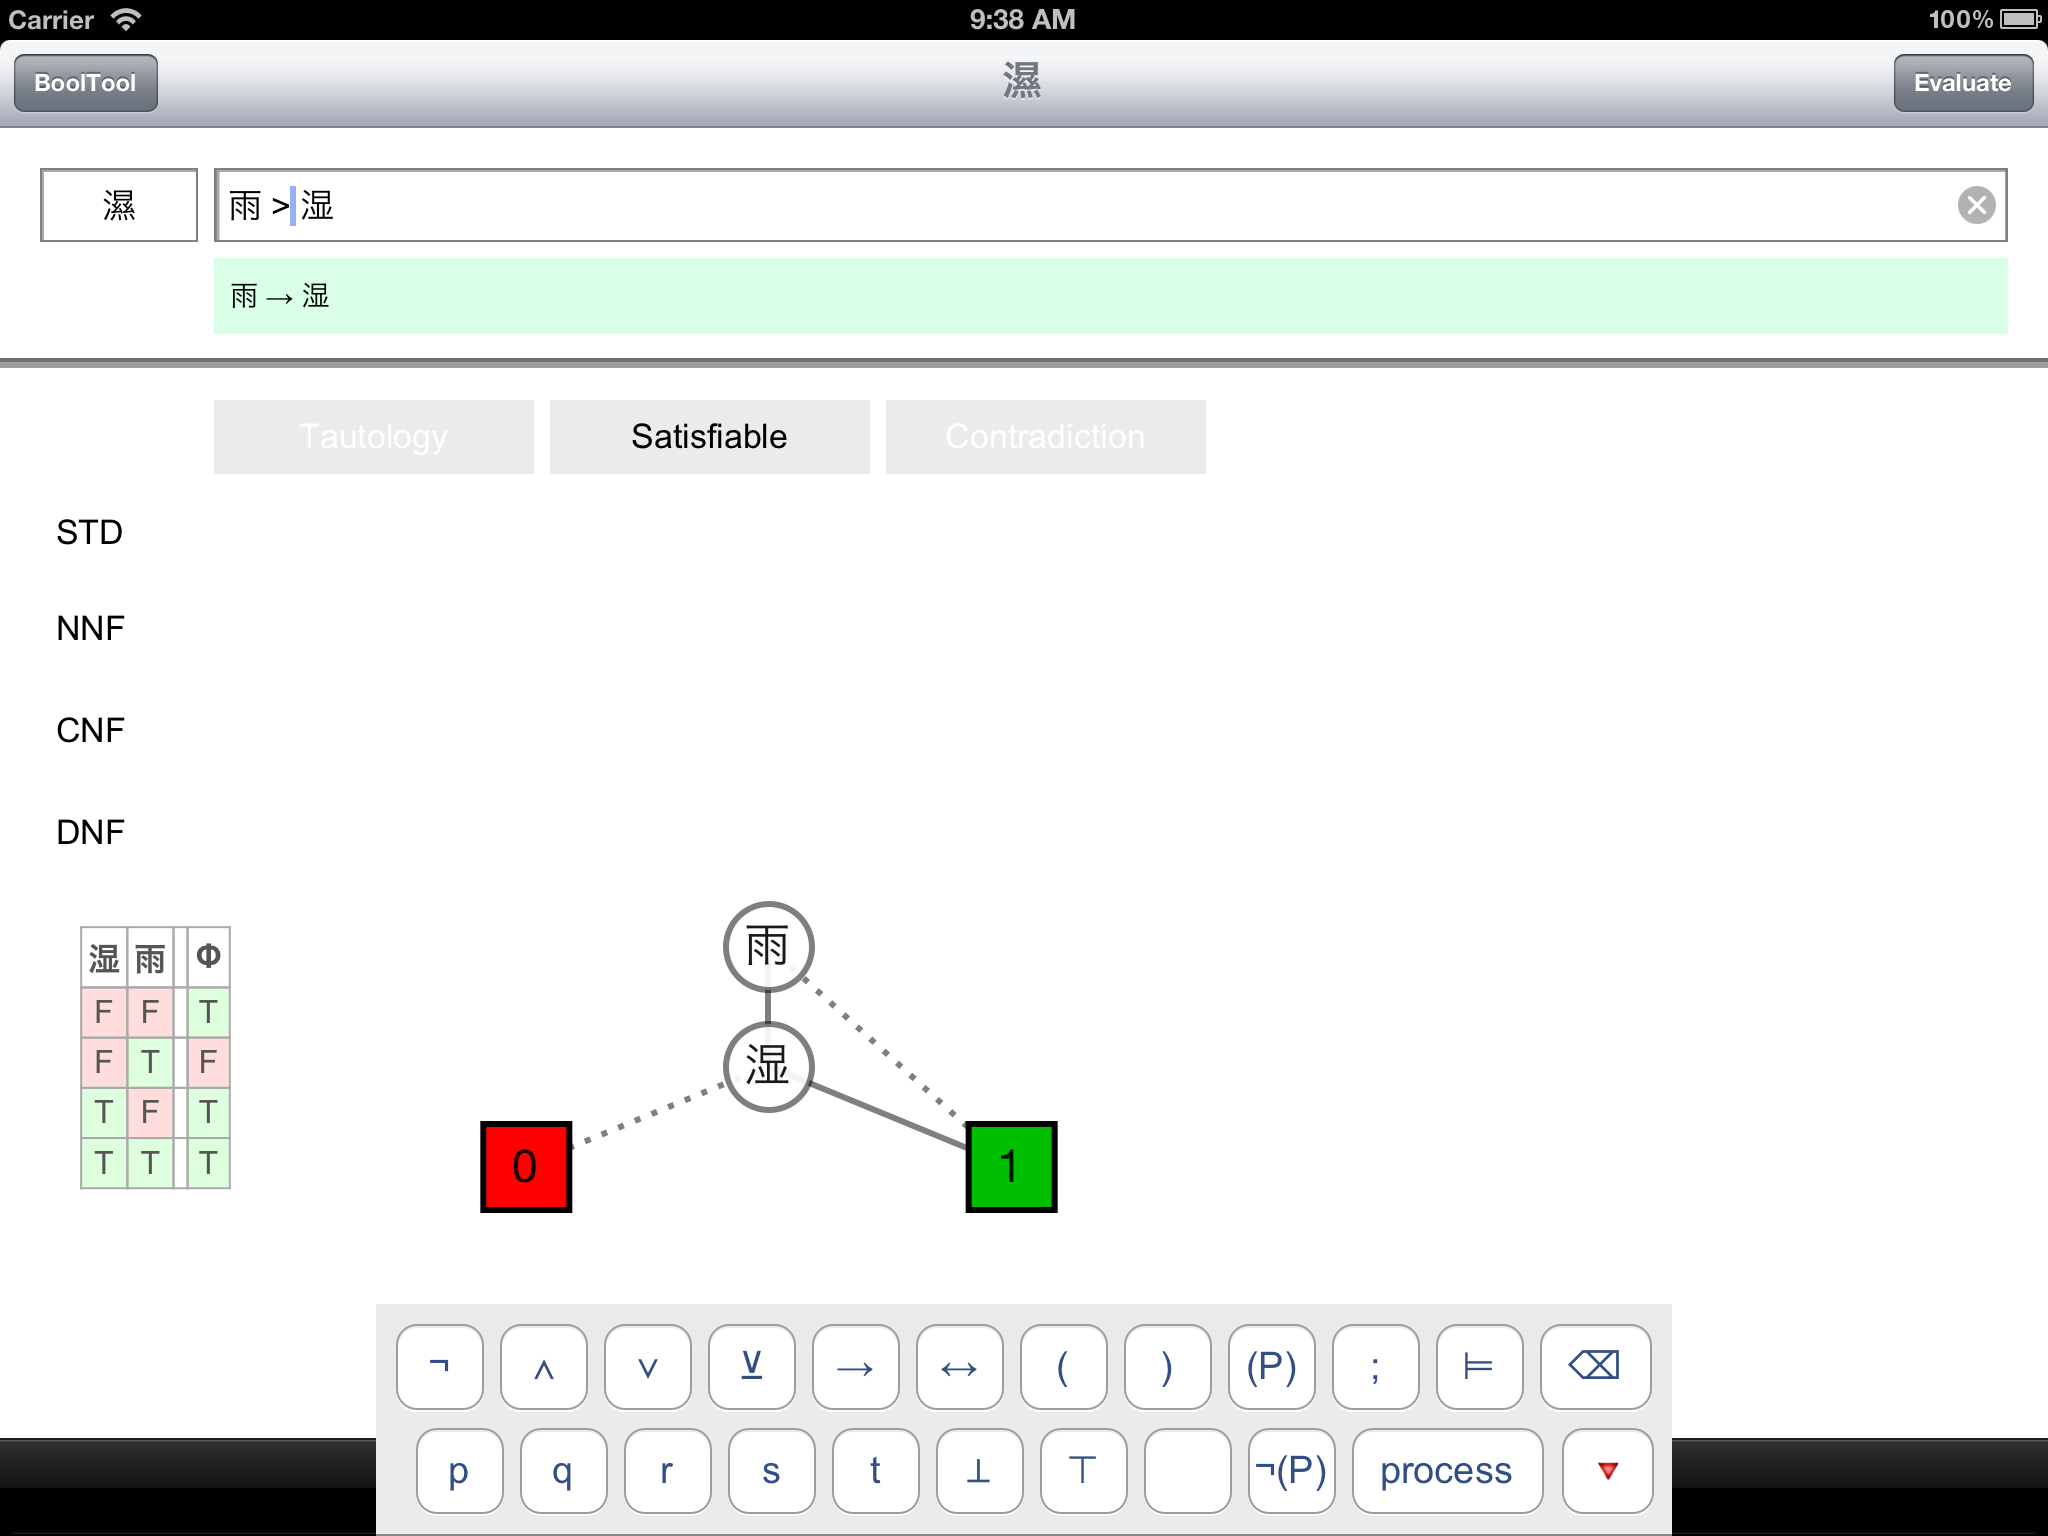
\includegraphics[scale=0.18,trim=0 43cm 0cm 0, clip=true]{concept/RainHD.png}
\caption{Implication with Chinese symbols for rain and wet}
\label{fig:BoolToolChineseInput}
\end{center}
\end{figure}

% ⊨|⊤|⊥|¬|!|∧|&|\\.|∨|\\+|\\||=|↔|<>|→|>|⊻|⊕|\\^|\\(|\\)|,|;|\\w+

\subsection{Output}

BoolTool calculates validity and satisfiability, 
conjunctive normal form, 
disjunctive normal form, 
truth table and 
(reduced) ordered binary decision diagram 
of user's input (\figref{fig:BoolToolROBDD}). 

\begin{figure}[htbp]
\begin{center}
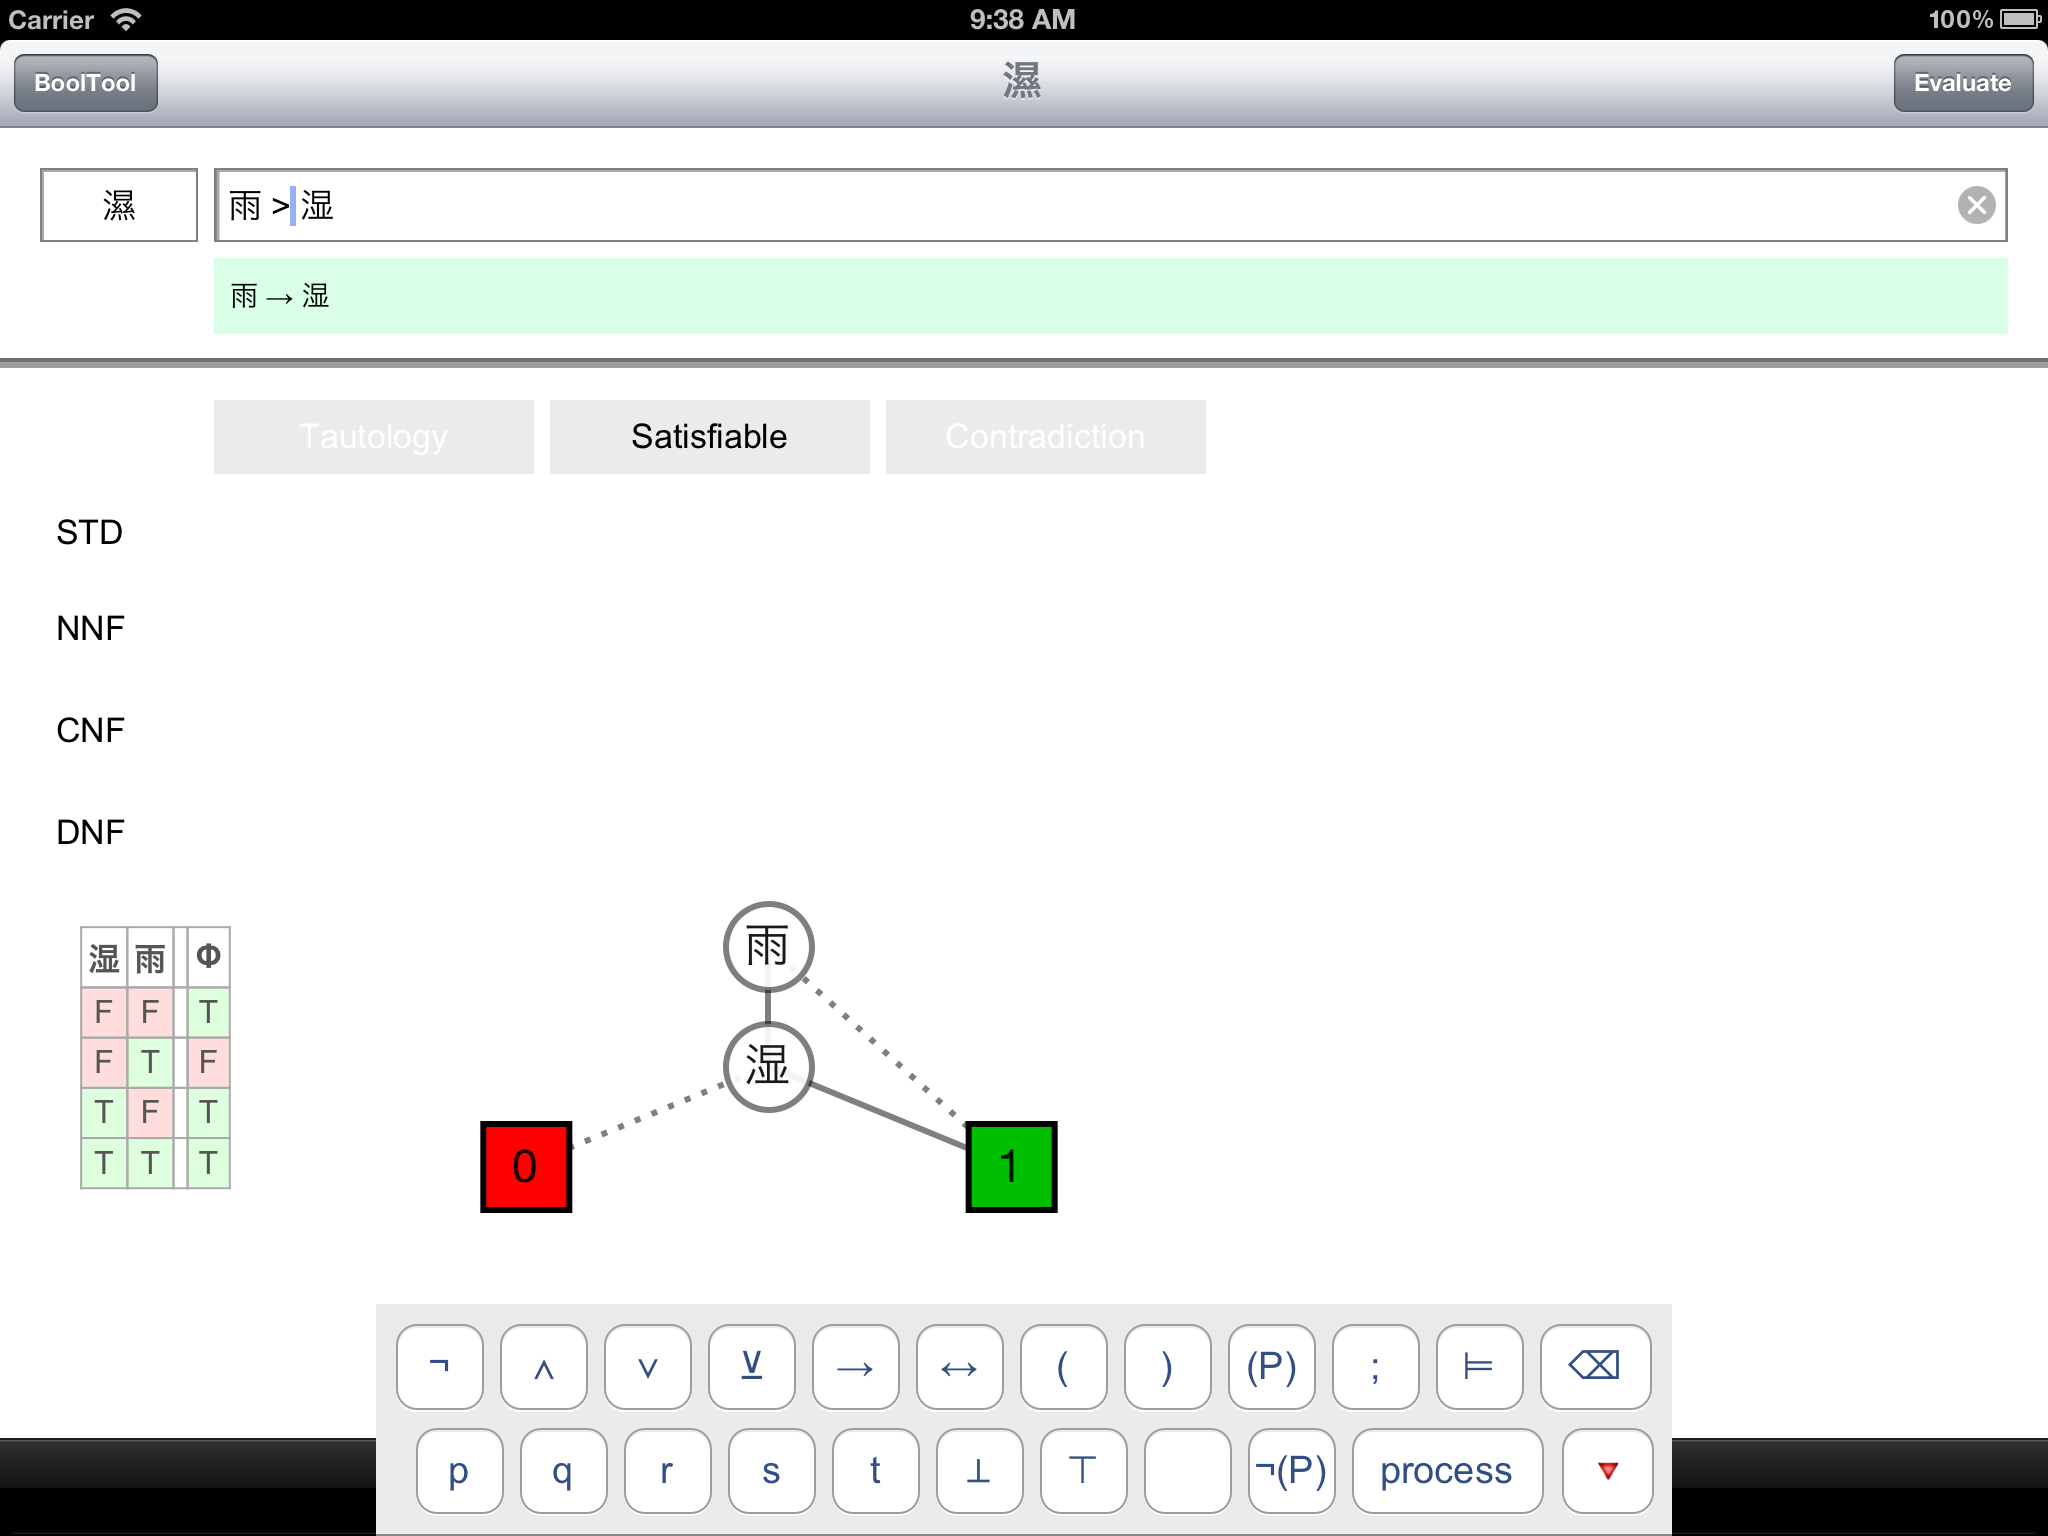
\includegraphics[scale=0.25,trim=16.5cm 11.4cm 34.5cm 31.8cm, clip=true]{concept/RainHD.png}
\caption{Reduced ordered binary decision diagram}
\label{fig:BoolToolROBDD}
\end{center}
\end{figure}

%\begin{figure}[htbp]
%\begin{center}
%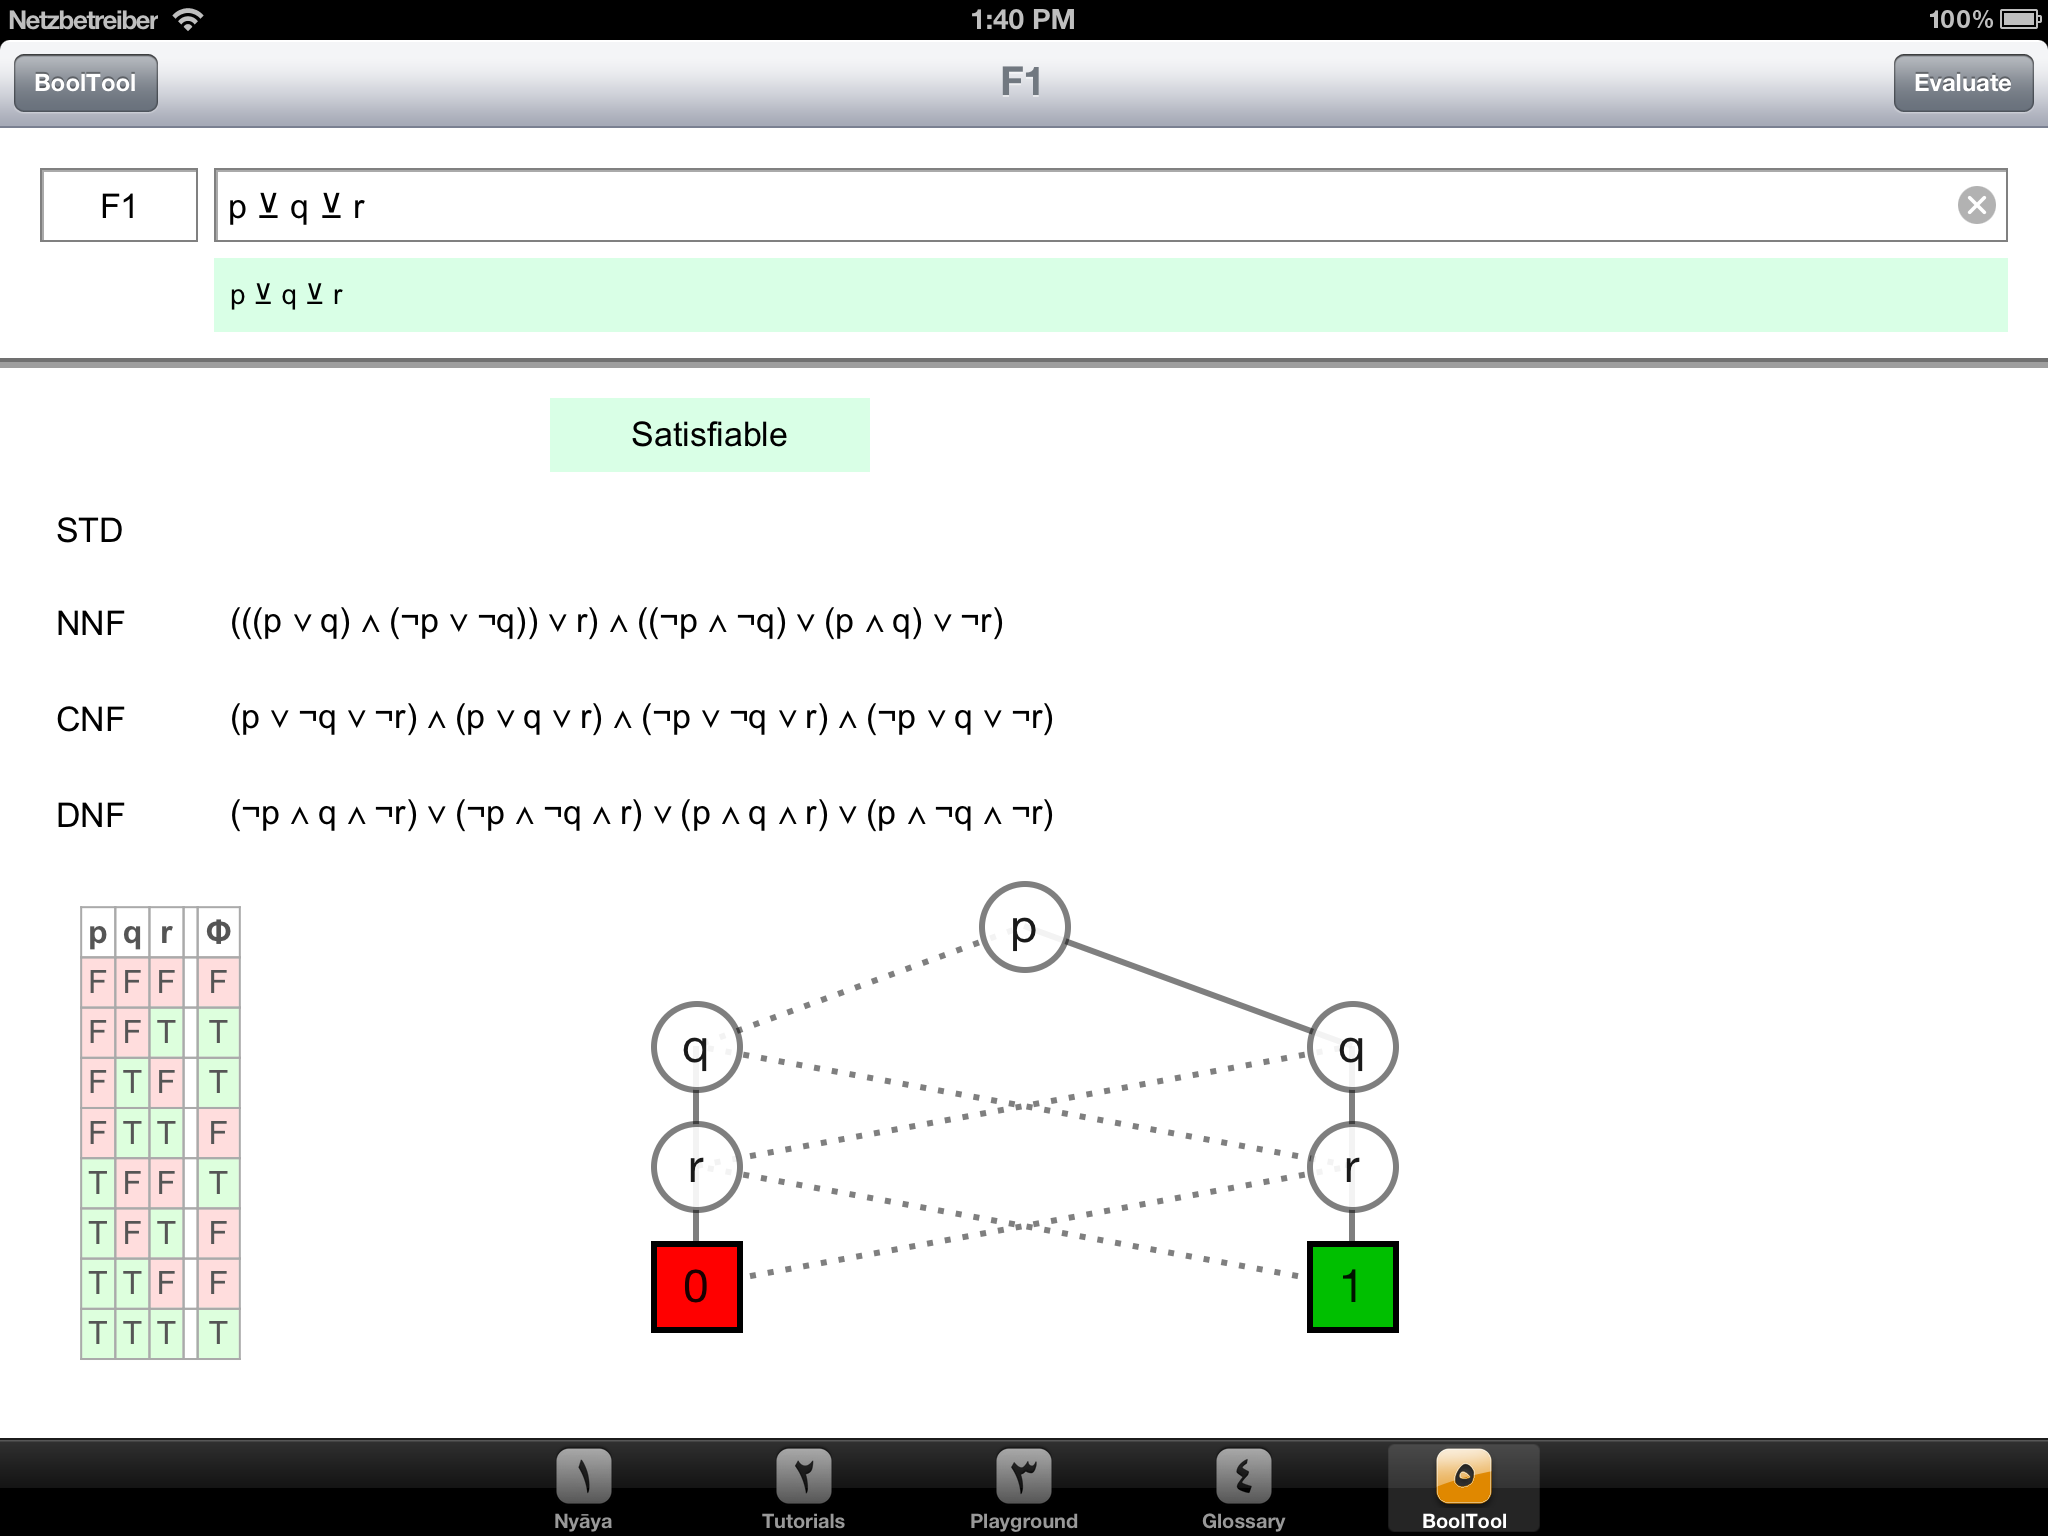
\includegraphics[width=13cm]{concept/BoolTool.png}
%\caption{Boolean function $p \oplus q \oplus r$}
%\label{fig:BoolToolOutput}
%\end{center}
%\end{figure}



